\section{Unconstrained MPC}\label{chap3}

Goal:Guarantee stability + degree of suboptimality
without stabilizing terminal constraint + cost

Setup: 
\begin{itemize}
\item $\dot x = f(x,u), x(0)=x_0$
\item input constraints $u(t) \in \mathbb{U} \subseteq \mathbb{R}^m \ \forall t \geq 0$
\end{itemize}

Infinite-horizon cost function:
$J_{\infty}(x_0, \bar{u}(\cdot; 0)) = \int_{0}^{\infty}L(\bar x(\tau;0), \bar u(\tau;0))d\tau  \Rightarrow$ optimal value function $J_{\infty}^*(x_0)$

Assumption: $J^{*}_{\infty}(x_0) < \infty, \forall x_0 \Rightarrow$ system is asymptotically stabilizable

Finite-horizon cost function:
$J_{T}(x(t), \bar{u}(\cdot; t)) = \int_{0}^{T}L(\bar x(\tau;t), \bar u(\tau;t))d\tau$

Infinite-horizon performance resulting from application of MPC controller:

$J_{\infty}^{MPC}(x_0) = \int_{0}^{\infty}L(\bar x_{MPC}(\tau), \bar u_{MPC}(\tau))d\tau$

\begin{Definition}
Suboptimality index $\alpha$:
$\alpha J_{\infty}^{MPC}(x_0) \leq J_{\infty}^{*}(x_0) \forall x_0$

\begin{itemize}
\item $\alpha \leq 1$ by optimality of $J^{*}_{\infty}$
\item $\alpha > 0$ implies closed-loop stability (Barb.lemma)
\end{itemize}
\end{Definition}

Proposition 1: Relaxed dynamic programming
 
Assume $\exists \alpha \in (0,1] s.t. \forall x \in \mathbb{R}^n$

$J_{T}^{*}(x(t+\delta)) \leq J_T^*(x(t)) - \alpha\int_{t}^{t+\delta}L(\bar x^*(\tau;t),\bar u^*(\tau;t))d\tau \ \ \ (*)$

Then the estimate 
\begin{equation}\label{main_inequility}
\alpha J_{\infty}^*(x(t)) \leq \alpha J_{\infty}^{MPC}(x(t)) \leq J_T^*(x(t)) \leq J_{\infty}^*(x(t))
\end{equation}

holds for all $x \in \mathbb{R}^n$

\begin{proof}
\begin{itemize}
\item 1 and 3 inequalities follow from optimality (by definition)
\item 2 inequality follows from summing up (*) over all sampling instances
\begin{equation}
J^*_T(x(N\delta)) \leq J_T^*(x_0) - \alpha \int_0^{N\delta}L(\bar x_{MPC}(t), \bar u_{MPC}(t))dt
\end{equation}
\begin{equation}
N \to \infty : J_T^*(x_0) \geq \alpha J_{\infty}^{MPC}(x_0) 
\end{equation}
\end{itemize}
\end{proof}

Central idea
\begin{center}
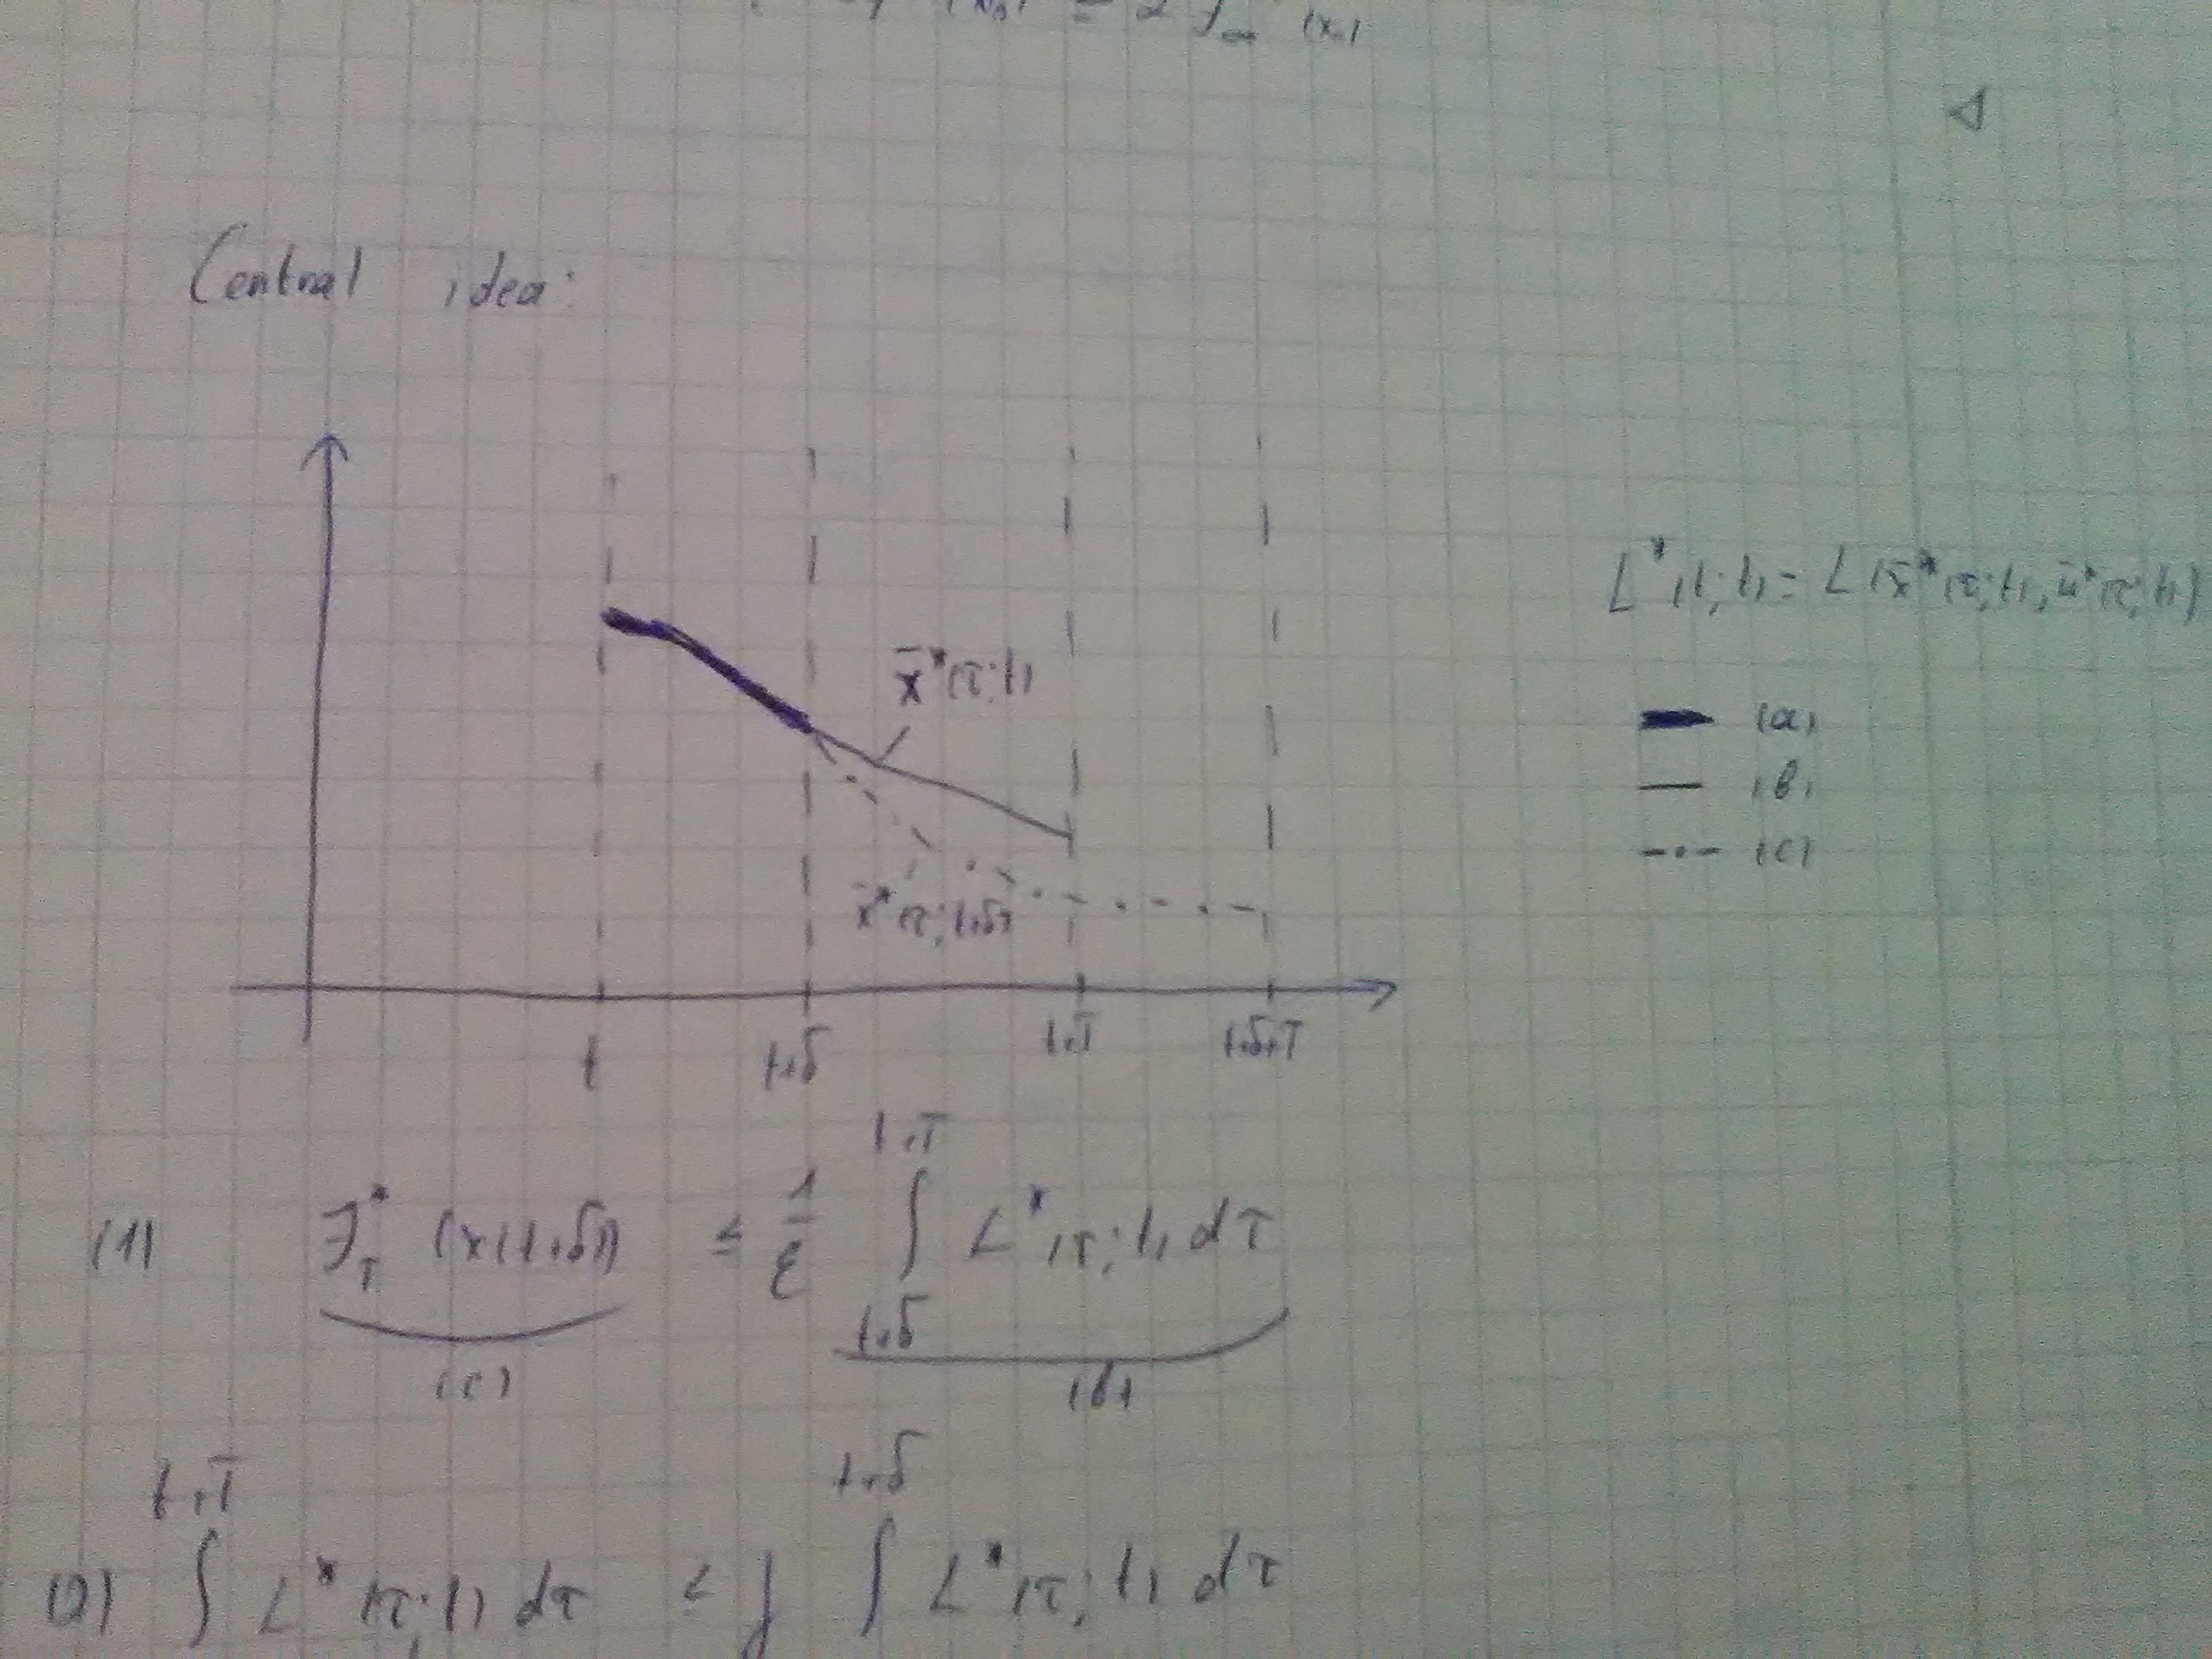
\includegraphics[scale=0.1]{1}
\end{center}

$L^*(\tau;t) = L(\bar x^*(\tau;t), \bar u^*(\tau;t))$

\begin{equation}\label{c_b_inequality}
(c): J_T^*(x(t+\delta)) \leq \frac{1}{\epsilon} \int_{t+\delta}^{t+T}L^*(\tau;t)d\tau :(b)
\end{equation}
\begin{equation}\label{b_a_inequality}
(b): \int_{t+\delta}^{t+T}L^*(\tau;t)d\tau \leq \gamma \int_{t}^{t+\delta}L^*(\tau;t)d\tau :(a)
\end{equation} 

\begin{Theorem}

Assume $\exists \epsilon \in (0;1]$ and $\gamma > 0$ s.t. \ref{c_b_inequality} - \ref{b_a_inequality} holds. Then (*) holds with $\alpha =1 - \gamma \frac{1-\epsilon}{\epsilon}$

\begin{proof}
\begin{equation*}
J_T^*(x(t+\delta)) - J_T^*(x(t)) = J_T^*(x(t+\delta)) - \int_{t}^{t+T}L^*(\tau;t)d\tau \leq^{(\ref{c_b_inequality})}
\end{equation*}
\begin{equation*}
\leq \frac{1-\epsilon}{\epsilon} \int_{t+\delta}^{t+T}L^*(\tau;t)d\tau - \int_t^{t+\delta}L^*(\tau;t)d\tau \leq^{(\ref{b_a_inequality})}
\end{equation*}
\begin{equation*}
\leq (\gamma \frac{1-\epsilon}{\epsilon} - 1) \int_t^{t+\delta}L^*(\tau;t)d\tau
\end{equation*} 
$-\alpha := \gamma \frac{1-\epsilon}{\epsilon} - 1$ 
\end{proof}
\end{Theorem}

Assumption 1: Asymptotic Controlability

For all $x_0$, $\exists$ some input trajectory $\hat u_x(\cdot)$
with $\hat u_x(t) \in \mathbb{U}, \forall t \geq 0$ s.t.
\begin{equation*}
L(\hat x(t),\hat u(t)) \leq \beta(t) \min_u L(x_0,u), \forall t > 0
\end{equation*}
with $\beta: \mathbb{R} \to \mathbb{R}_{\geq 0}$
 - continuous, positive, strictly decreasing with $\lim_{t \to 0} \beta(t) = 0$ $\Rightarrow$
$\int_0^{\infty}\beta(\tau)d\tau < \infty$
$B(t) = \int_0^t\beta(\tau)d\tau$

Typical example:
\begin{center}
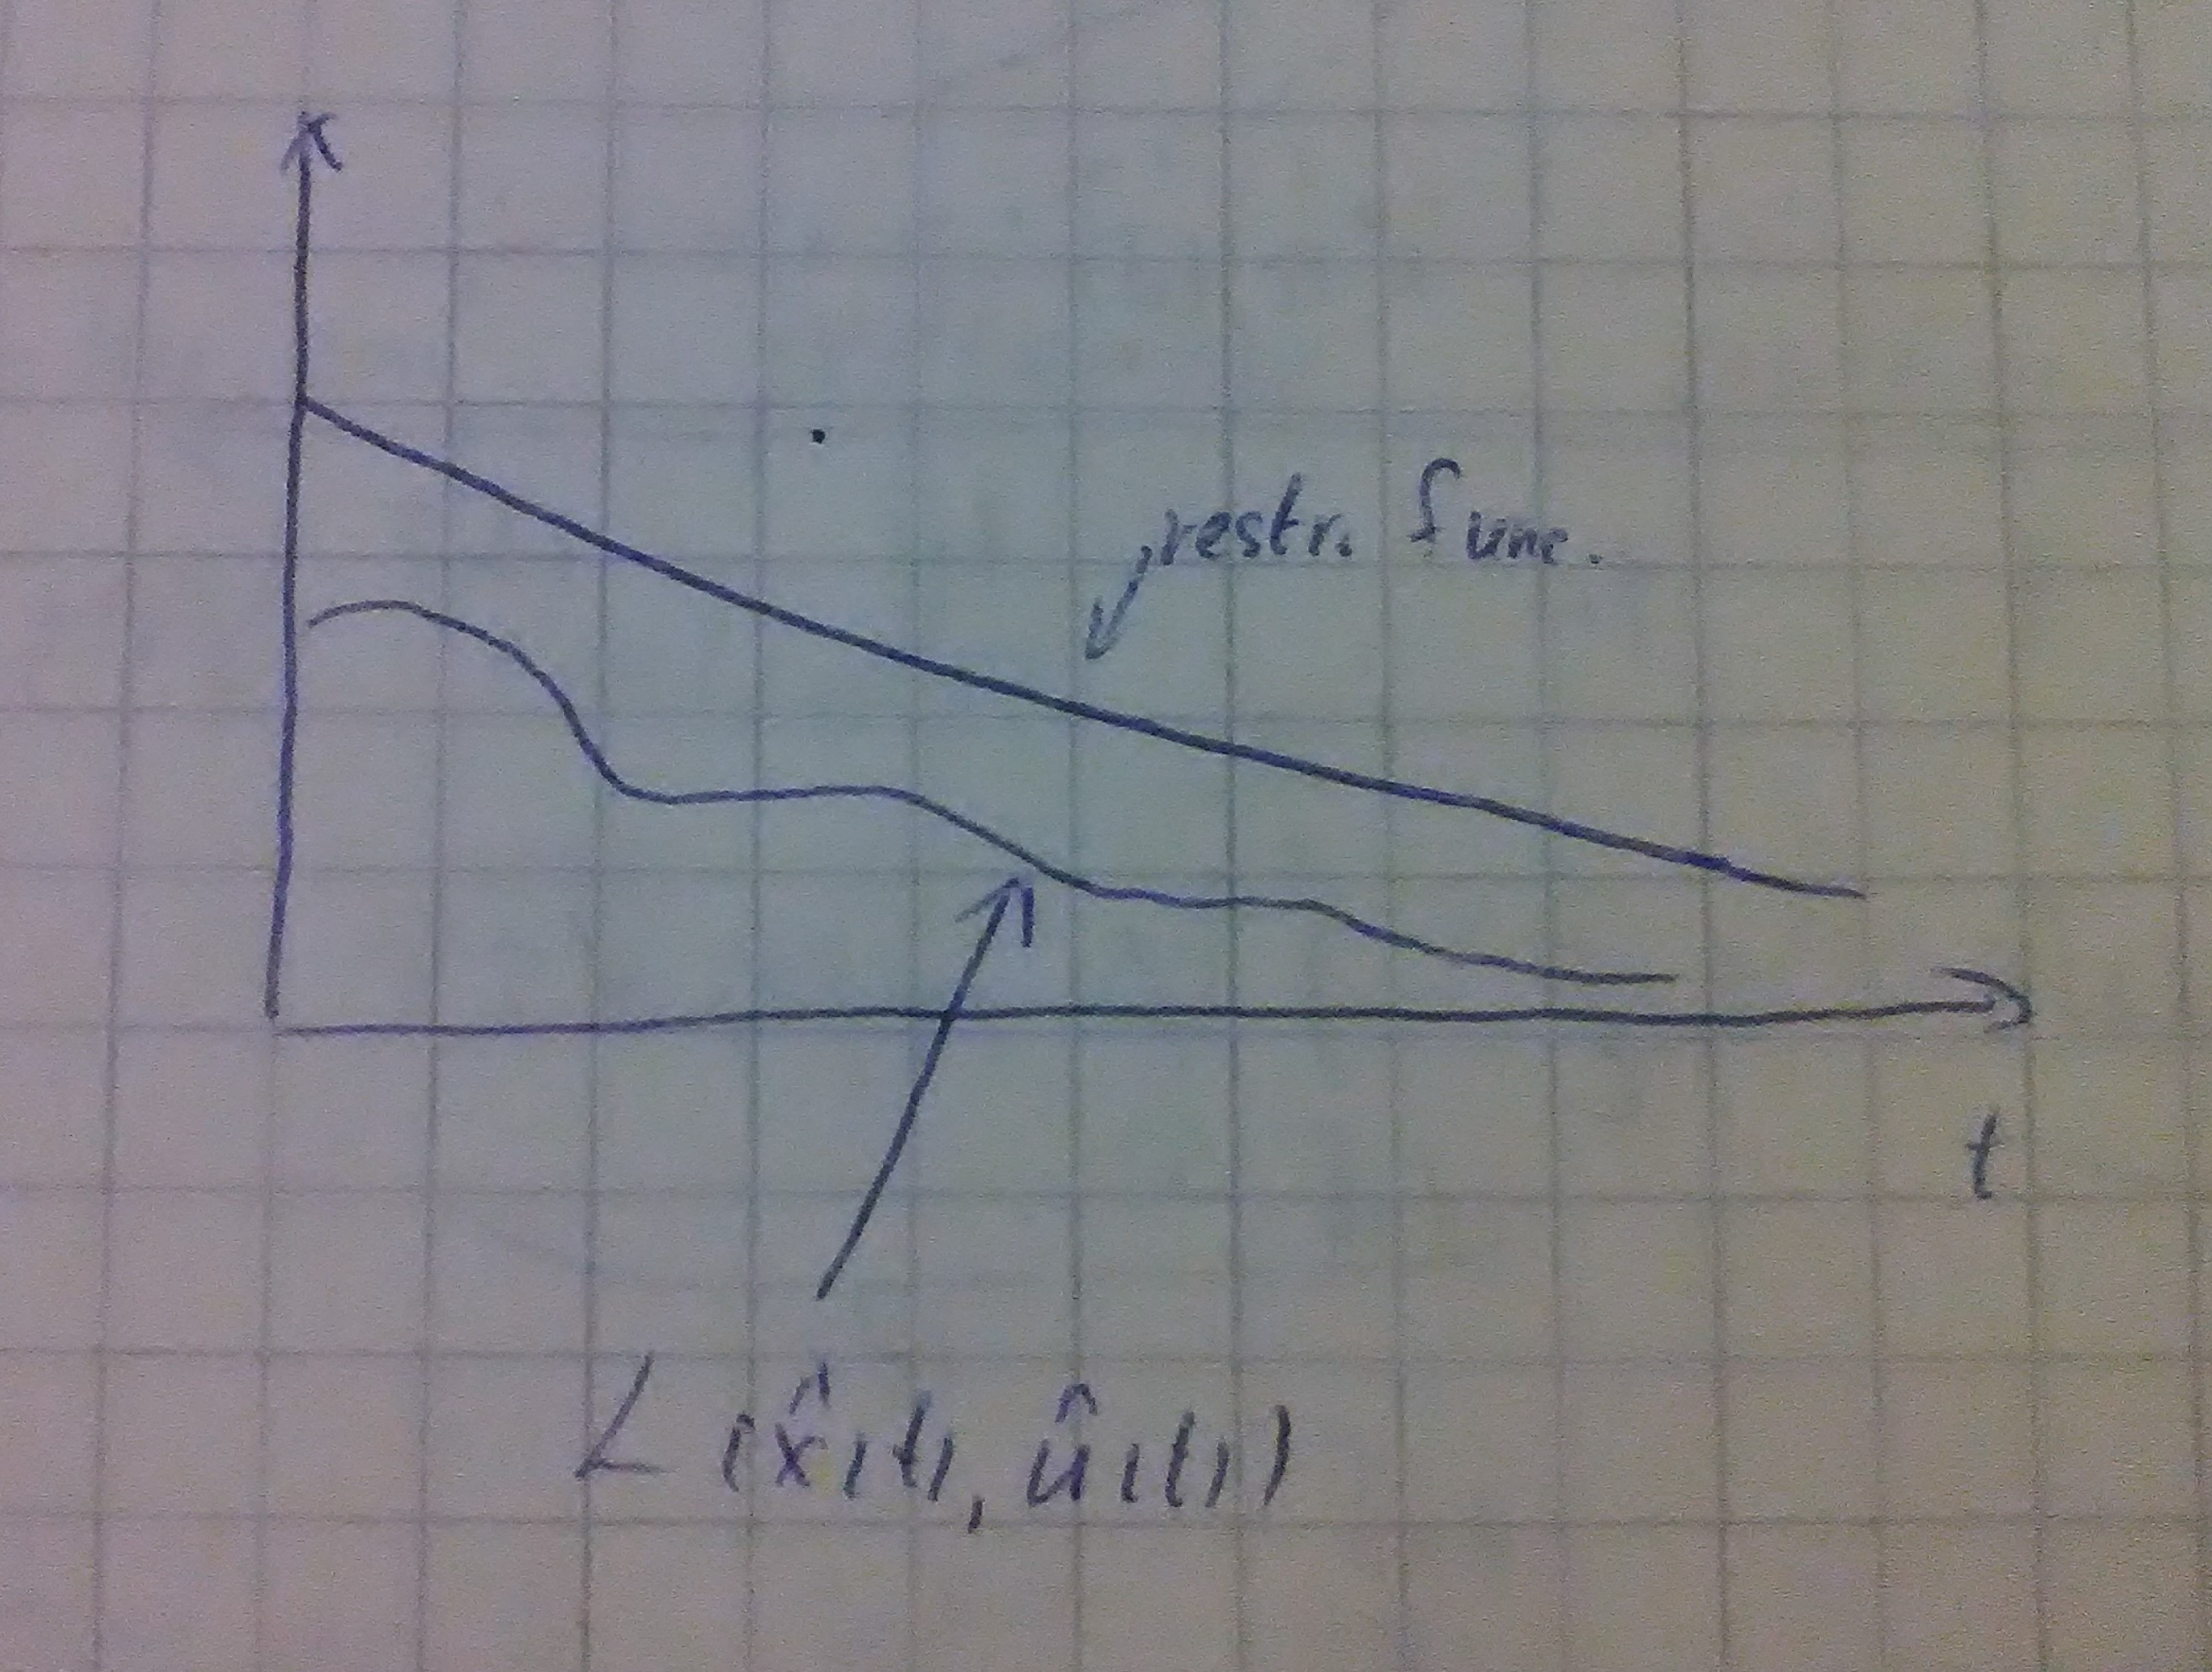
\includegraphics[scale=0.1]{2}
\end{center}

How to compute $\epsilon$ and $\gamma$:
\begin{Lemma} 
Let Assumption 1 hold. Then the inequality 
\begin{equation}\label{lemma_1_inequality}
J_T^*(x(t+\delta)) \leq \int_{t+\delta}^{t+t'}L^*(\tau;t)d\tau + B(T+\delta - t')L^*(t+t';t)
\end{equation}
holds for all $t' \in [\delta,T]$

(image to be inserted)


\begin{proof}

Consider 
\begin{equation*}
\bar u(\tau;t+\delta) = \left \{
  \begin{tabular}{c}
  $\bar u^*(\tau;t), \tau \in [t+\delta, t+t']$ \\
  $\hat u_{x'}(\tau - t - t'), \tau \in [t+t', t+\delta + T]$
  \end{tabular}
\right.
\end{equation*}
\begin{equation*}
J^*_T(x(t+\delta)) \leq J_T(x(t+\delta), \bar u(\cdot;t+\delta)) =
\end{equation*}
\begin{equation*}
=\int^{t+t'}_{t+\delta}L^*(\delta;t)d\delta + \int_{t+t'}^{t+\delta+T}L(\hat x(\tau - t - t'), \hat u (\tau - t - t'))d\tau \leq
\end{equation*} 
by Assumption 1
\begin{equation*}
\int_{t+t'}^{t+\delta+T}L(\hat x(\tau - t - t'), \hat u (\tau - t - t'))d\tau \leq L^*(t+t';t) \int_0^{T+\delta-t'}\beta(\tau)d\tau
\end{equation*}
as far as $B(t) = \int_0^t\beta(\tau)d\tau$
\begin{equation*}
\leq \int_{t+\delta}^{t+t'}L^*(\tau;t)d\tau + B(T+\delta-t')L^*(t+t';t)
\end{equation*}
\end{proof}
\end{Lemma}

Calculation of $\epsilon$ from (\ref{lemma_1_inequality}):
\begin{equation*}
J^*_T(x(t+\delta)) \leq \min_{t' \in [\delta,T]}(\int_{t+\delta}^{t+t'}L^*(\tau;t)d\tau + B(T+\delta-t')L^*(t+t';t)) \leq
\end{equation*}
\begin{equation*}
\int_{t+\delta}^{t+T}L^*(\tau;t)d\tau + B(T) \min_{t'\in[\delta,T]}L^*(t+t';t)
\end{equation*}
as far as 
$\min_{t'\in[\delta,T]}L^*(t+t';t) \leq \frac{1}{T-\delta}\int_{t+\delta}^{t+T}L^*(\tau;t)d\tau$
minimum is less or equal that the average
\begin{equation*}
=(1+\frac{B(T)}{T-\delta})\int_{t+\delta}^{t+T}L^*(\tau;t)d\tau
\end{equation*}
$(1+\frac{B(T)}{T-\delta}) = \frac{1}{\epsilon}$

\begin{Lemma}

\begin{equation*}
\int_{t+t'}^{t+T}L^*(\tau;t)d\tau \leq B(T-t')L^*(t+t';t) \forall t' \in [0;T]
\end{equation*}

\begin{proof}
Analogues to lemma 2.

Calculation of $\gamma$:

\begin{equation*}
\int_{t+\delta}^{t+T} L^*(\tau;t)d\tau \leq \int_{t+\hat t}^{t+T}L^*(\tau;t)d\tau (\forall \hat t \in [0,\delta]) \leq
\end{equation*}
\begin{equation*}
\leq \min_{\hat t \in [0, \delta]}(B(T-\hat t)L^*(t+\hat t;t)) \leq
\end{equation*}
\begin{equation*}
\leq B(T)\min_{\hat t \in [0,\delta]}L^*(t+\hat t;t) \leq \frac{B(T)}{\delta}\int_{t}^{t+\delta}L^*(\tau;t)d\tau
\end{equation*}
\end{proof}
\end{Lemma}

Denote $\gamma = \frac{B(T)}{\delta}$

$\alpha = 1 - \gamma \frac{1-\epsilon}{\epsilon} = 1 - \frac{B(T)}{\delta}(\frac{B(T)}{T-\delta})$

Alternative computation of $\epsilon$ (less conservative):

We want to compute $\epsilon$ s.t.
\begin{equation*}
\epsilon \leq \frac{\int_{t+\delta}^{t+T}L^*(\tau;t)d\tau}{J_T^*(x(t+\delta))}
\end{equation*}

Idea: Minimize 
\begin{equation}\label{minimizer_eps}
\epsilon = \min_{L_t,J^*_T}\frac{\int_{\delta}^{T}L_t(\tau;t)d\tau}{J_T^*(x(t+\delta))}
\end{equation}
$J^*_T = 1$ - without loss of generality
s.t. $0 \leq L_t \ \forall \tau \in [\delta,T]$
\begin{equation*}
J^*_T(x(t+\delta)) \leq \int_{\delta}^{t'}L_t(\tau)d\tau + B(T+\delta-t')L_t(t') \forall t' \in [\delta, T]
\end{equation*}
Due to linearity in $L_t$, without loss of generality we can set $J_T^* = 1$.

$\Rightarrow$ infinite dimensional linear problem

Idea for solution:
second constraint has to be active for all times 

Differentiate (\ref{lemma_1_inequality}) with relation to $t'$ 
\begin{equation*}
0 = L_t(t') + \frac{dB(T+\delta-t')}{dt'}L_t(t') + B(T + \delta - t') \dot L_t(t')
\end{equation*} 
as far as $\frac{dB(T+\delta-t')}{dt'} = -\beta(T+\delta - t')$

\begin{equation*}
\left \{
  \begin{tabular}{c}
  $\dot L_t(t') = \frac{\beta(T+\delta - t') -1}{B(T+\delta - t')}L_t(t')$ \\
 initial condition $L_t(\delta)=\frac{1}{B(T)}$
  \end{tabular}
\right .
\end{equation*}

Solution:
\begin{equation*}
\bar L_t(t') = \frac{1}{B(T+\delta-t')}e^{-\int_{\delta}^{t'}\frac{1}{B (T+\delta-\tau)}d\tau}
\end{equation*}
Have to show: $\bar L_t$ is a minimizer of (\ref{minimizer_eps})
\begin{equation*}
\int_{\delta}^{T} \bar L_t(\tau)d\tau \leq \int_{\delta}^{T} L_t(\tau)d\tau 
\end{equation*}
for all feasible $L_t$

\begin{proof}

Assume $\exists L_t$ s.t. 
\begin{equation*}
\int_{\delta}^{T}L_t(\tau)d\tau < \int_{\delta}^{T}\bar L_t(\tau)d\tau
\end{equation*}
Then $\exists \hat t \in [\delta, T]$ s.t. $\int_{\delta}^{\hat t}L_t(\tau)d\tau \leq \int_{\delta}^{\hat t}\bar L_t(\tau)d\tau$ and $\bar L_t(\hat t) > L_t(\hat t)$

But then 
\begin{equation}
1 = \int_{\delta}^{\hat t} \bar L_t(\tau)d\tau + B(T+\delta-\hat t)\bar L_t(\hat t) > \int_{\delta}^{\hat t}L_t(\tau)d\tau + B(T+\delta-\hat t) L_t(\hat t)
\end{equation}

the sign equality from (\ref{minimizer_eps}) with equality.

Contradiction:

$L_t$ cannot be a feasible solution of (\ref{minimizer_eps}) 
$\Rightarrow$ 
\begin{equation*}
\epsilon = \int_{\delta}^{T}\bar L_t(\tau)d\tau = 1 - e^{-\int_0^{T-\delta}\frac{1}{B(T-\tau)}d\tau}
\end{equation*}
\end{proof}
Similarly, better estimate for $\gamma$ can be obtained

$\alpha = 1 - \gamma\frac{1-\epsilon}{\epsilon}$
For $T \to \infty$ : both estimates for $\epsilon \to 1 \Rightarrow \alpha \to 1$ as $T \to \infty \Rightarrow$ closed-loop stability for $T$ large enough 
